\documentclass[11pt]{article}
\usepackage[margin=1in]{geometry}
\usepackage{amsmath,amssymb,amsthm}
\usepackage{graphicx}
\usepackage{microtype}
\usepackage[hidelinks]{hyperref}

\newtheorem{theorem}{Theorem}

\title{Counit Edge-Case Counterexamples for Two Ideal Questions\\
\large Candidate negative answers to Questions 5.3 and 5.4 of arXiv:2111.13247}
\author{Automated mathematical discovery run \texttt{fa\_banach\_001}, lane 15}
\date{11 August 2026}

\begin{document}
\maketitle

\begin{center}
\fbox{\parbox{0.91\linewidth}{\textbf{Status.} Candidate full
counterexamples to the questions as written, likely valid, requiring expert
review. The construction uses the permitted zero-ideal edge case.}}
\end{center}

\begin{abstract}
Questions 5.3 and 5.4 of Anderson-Sackaney have negative answers as stated.
Let $\mathbb G$ be a noncoamenable compact quantum group and take the
contractive convolution idempotent to be its universal counit
$\epsilon_{\mathbb G}^u$. Its multiplier is the identity, so the associated
compact quasi-subgroup is all of $L^\infty(\mathbb G)$ and both ideals in the
questions are zero. The zero ideal has the constant-zero bounded right
approximate identity. On the other hand, the universal counit does not belong
to the reduced measure algebra, since that would give a reduced counit and
coamenability. The compact dual of the free group $\mathbb F_2$ gives a
concrete example. Proper/nonzero variants are not settled.
\end{abstract}

\section{The two source questions}

The source asks whether a brai for $J^1(N)$ forces the idempotent state
$\omega_N$ to belong to $M^r(\mathbb G)$, and more generally whether the
preannihilator of the range of every contractive-idempotent multiplier has a
brai exactly when $\mathbb G$ is coamenable \cite{source}.

\begin{figure}[ht]
  \centering
  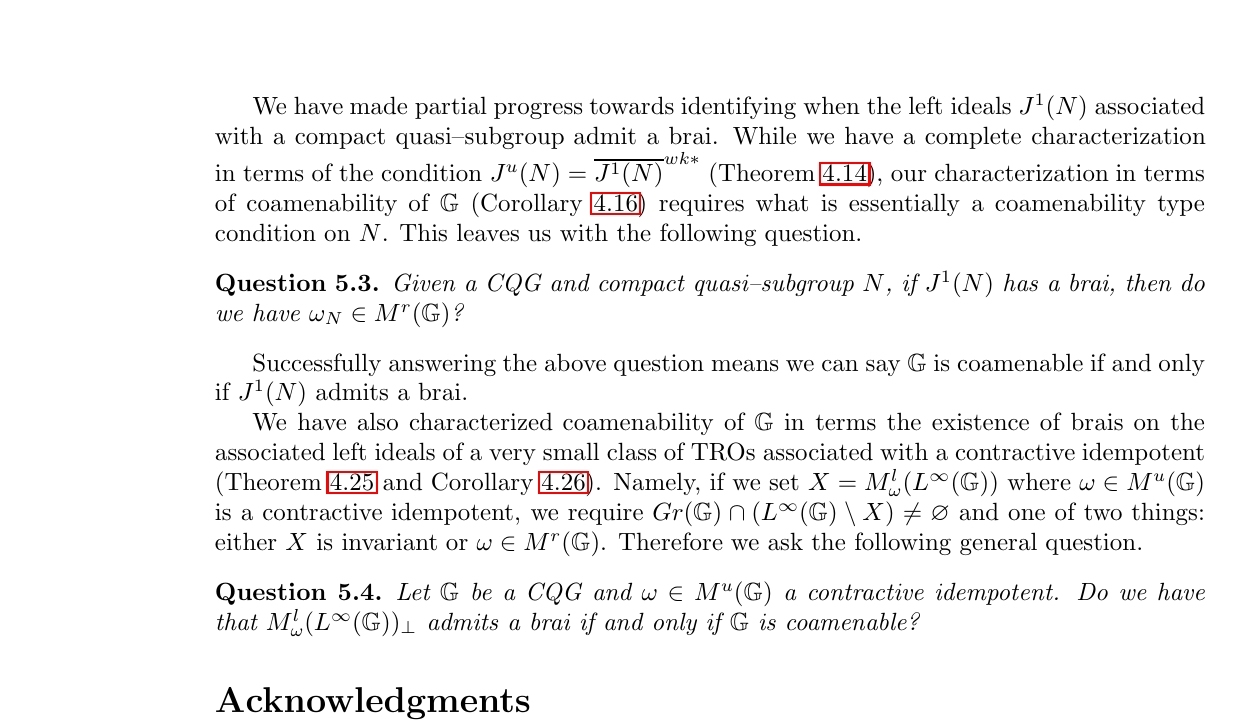
\includegraphics[width=0.96\linewidth]{figures/questions_5_3_5_4_crop.png}
  \caption{Questions 5.3 and 5.4 in the source, PDF p.~30.}
\end{figure}

\section{Counterexample}

\begin{theorem}\label{thm:main}
Questions 5.3 and 5.4 of \cite{source} are both false as written.
\end{theorem}

\begin{proof}
Let $\Gamma=\mathbb F_2$ and let $\mathbb G=\widehat\Gamma$ be its compact
dual quantum group. Thus
\[
 C^u(\mathbb G)=C^*(\Gamma),\qquad
 C^r(\mathbb G)=C_r^*(\Gamma).
\]
The compact quantum group $\mathbb G$ is not coamenable because $\Gamma$ is
not amenable \cite{bedos}.

Let $\epsilon_{\mathbb G}^u\in M^u(\mathbb G)=C^u(\mathbb G)^*$ be the
universal counit. It is a unital character and hence a norm-one state. It is
also the convolution unit, so
\[
 \epsilon_{\mathbb G}^u*\epsilon_{\mathbb G}^u
 =\epsilon_{\mathbb G}^u.
\]
It is therefore a contractive idempotent of precisely the kind allowed in
Question 5.4. The counit identity gives
\[
 M^l_{\epsilon_{\mathbb G}^u}=\operatorname{id}_{L^\infty(\mathbb G)},
\]
an identity also recorded in the source's multiplier preliminaries.

Under the source's correspondence between idempotent states and compact
quasi-subgroups, $\epsilon_{\mathbb G}^u$ corresponds to
\[
 N=M^l_{\epsilon_{\mathbb G}^u}(L^\infty(\mathbb G))
   =L^\infty(\mathbb G).
\]
Consequently
\[
 J^1(N)=N_\perp=\{0\}.
\]
The constant net $e_i=0$ is a bounded right approximate identity for this
ideal: the relation $f*e_i\to f$ is automatic for its sole element $f=0$.

However,
\[
 \epsilon_{\mathbb G}^u\notin M^r(\mathbb G).
\]
Indeed, membership in the embedded reduced measure algebra would make the
universal counit factor through the reducing morphism
$C^u(\mathbb G)\to C^r(\mathbb G)$. This supplies a reduced counit, which for
a compact quantum group is equivalent to coamenability, contradicting the
choice of $\mathbb G$.

Thus $J^1(N)$ has a brai although
$\omega_N=\epsilon_{\mathbb G}^u\notin M^r(\mathbb G)$, disproving Question
5.3. For Question 5.4, the relevant ideal is likewise
\[
 M^l_{\epsilon_{\mathbb G}^u}(L^\infty(\mathbb G))_\perp
 =L^\infty(\mathbb G)_\perp=\{0\},
\]
which has a brai although $\mathbb G$ is not coamenable. This disproves the
proposed equivalence.
\end{proof}

\section{Scope, verification, and novelty}

The counterexamples use no pathology beyond the convolution unit. They show
that the two universal statements need a nondegeneracy hypothesis. Natural
repairs include requiring $N\neq L^\infty(\mathbb G)$, requiring the ideal to
be nonzero, or requiring the multiplier range to be proper. The source's
earlier sufficient theorem uses an intrinsic-group element outside the
range, which automatically excludes this example. None of those repaired
questions is answered here.

The proof audit checks that the counit is an idempotent state, its multiplier
is the identity, the whole algebra is an allowed compact quasi-subgroup, the
zero ideal has a brai, and a reduced counit would force coamenability. No
computation is relevant.

A bounded search on 11 August 2026 covered the four run indexes, exact
question wording, the source title and arXiv id, the published version, the
author's thesis, counit/contractive-idempotent combinations, and later
citations. No explicit statement of this edge-case counterexample was found.
Novelty evidence is provisional.

\section*{Human-review recommendation}

Check the two conventions on which the edge case rests: the whole algebra is
not excluded from the source's compact quasi-subgroups, and the zero ideal is
allowed to have the constant-zero brai. Then verify the familiar equivalence
between descent of the universal counit and coamenability.

\begin{thebibliography}{9}
\bibitem{source}
B. Anderson-Sackaney,
\emph{On ideals of $L^1$-algebras of compact quantum groups},
Int. J. Math. \textbf{33} (2022), 2250074; arXiv:2111.13247,
Questions 5.3--5.4.

\bibitem{bedos}
E. B\'edos, G. J. Murphy, and L. Tuset,
\emph{Co-amenability of compact quantum groups},
J. Geom. Phys. \textbf{40} (2001), 130--153.
\end{thebibliography}

\end{document}
